%
% 「降臨鉄道」インタラクション2015ポスタ
%
% 山田尚昭 and 増井俊之
% 2014/12/13 17:40:18
%
% 以下を eval-region して句読点設定
% (replace-string "。" ".")
% (replace-string "、" ",")
%

\documentclass[submit,techreq]{ipsj}

\usepackage[dvipdfmx]{graphicx}

\usepackage{latexsym}
\usepackage{here} % [H]とするとその場所に配置される

% ???
\def\Underline{\setbox0\hbox\bgroup\let\\\endUnderline}
\def\endUnderline{\vphantom{y}\egroup\smash{\underline{\box0}}\\}
\def\|{\verb|}

% インタラクション特有の設定.印刷工程で柱・ノンブルの埋め込みを行う.
\makeatletter
\pagestyle{empty}
\def\@oddhead{}
\def\@evenhead{}
\def\ps@IPSJTITLEheadings{}
\makeatother

\begin{document}

\title{降臨鉄道: 模型モノレールを利用した遠隔通信}
\etitle{Camera on Rails: Telecommunication with Model Monorail Trains}

\affiliate{KU}{慶應義塾大学 環境情報学部\\
Faculty of Environment and Infomation Studies, Keio University}

\affiliate{MG}{慶應義塾大学大学院 政策・メディア研究科\\
Graduate School of Media and Governance, Keio University}

\author{山田 尚昭}{Naoaki Yamada}{KU}
\author{中山 拓哉}{Takuya Nakayama}{KU}
\author{橋本 翔}{Sho Hashimoto}{MG}
\author{増井 俊之}{Toshiyuki Masui}{KU}

\begin{abstract}
カメラを登載した模型モノレールをオフィスの天井で走らせることによって,
どこからでもオフィスの様子を覗いたりオフィス内の人間と会話したりできる遠隔通信システムを作成した.
床を移動するロボットを利用することによって
遠隔地のユーザが会議や学会に参加する試みが近年盛んになっているが,
混雑した環境ではロボットが自由に移動できないため実運用が難しいことが多い.
邪魔物が無い天井に装着したレール上を自由に動けるモノレールを利用することにより,
実用的な遠隔コミュニケーションシステムが実現できた.
\end{abstract}

\begin{eabstract}
We developed the ``Camera on Rails'' telecommunication system with
which a user can communicate with other people in a
distance office through a camera on a model monorail train running on the ceiling
of the office. Using our system, the user can monitor the current status
of the office by running the train on the ceiling and have
conversation with the people in the office.
% from arbitrary angles.
\end{eabstract}

\maketitle

\section{はじめに}

遠隔地の人と同じ場所にいるかのような感覚を強化する
テレプレゼンスシステムの研究が盛んであり、
ビデオ会議システムや遠隔操作可能なロボットなどが普及しつつある.
%
2014年に開催されたWISS2014では、
Double RoboticsのDouble\footnote{
  \textsf{http://www.doublerobotics.com}
}というテレプレゼンスロボットの導入により、
遠隔地の人間が会議に参加可能になっていた(図\ref{double})\footnote{
  \textsf{http://engineer.typemag.jp/article/yuki-igarashi41}
}。

\begin{figure}[t]
\centerline{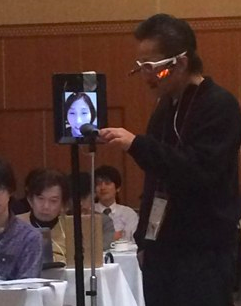
\includegraphics[width=40mm]{figures/b74f4564d4b38d12e48fcf80fef96def.png}}
\caption{Doubleを利用した質疑応答.}
\label{double}
\end{figure}

筆者の研究室では、卓上を動き回ることのできる
ガンタンク\footnote{
  「機動戦士ガンダム」に登場する有人式人型ロボット兵器。
}のプラモデルを利用した遠隔コミュニケーション支援システム「OB降臨システム」を
作成して運用しているが\cite{Hirota:Korin},
ケーブルの制約のため動ける範囲が狭く、
机の上の障害物のために移動が制限されたりカメラからの映像が見られなかったり
することが多かった(図\ref{guntank}).

\begin{figure}[H]
\centerline{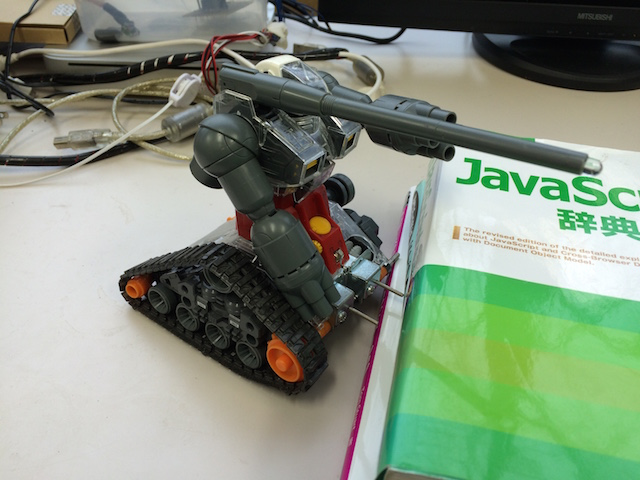
\includegraphics[width=50mm]{figures/1e8781bb2a5b28c8e06906d226c7505a.png}}
\caption{動きがとれなくなっているガンタンク.}
\label{guntank}
\end{figure}

邪魔物が存在しない天井を移動する遠隔情報共有システム「降臨鉄道」を提案する.



% \section{関連研究}
%
% \begin{figure}[H]
% \centerline{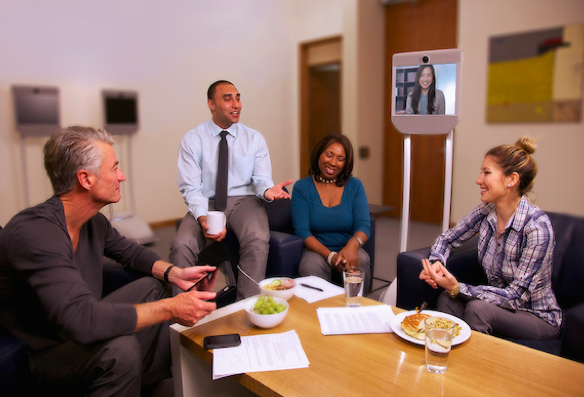
\includegraphics[width=60mm]{figures/2c092d5d4467d5b2572acef0c95b22ff.png}}
% \caption{BeamPro.}
% \label{beampro}
% \end{figure}
%
% \footnote{
%   \textsf{https://www.suitabletech.com/beam/}
% }
%
% Jouppiのシステム\cite{Jouppi:2002:FST:587078.587128}では自由に動き回れるロボットで遠隔地を訪れられる.大掛かりな
% 操作室が必要だが,現地での活動能力は高い.

\section{降臨鉄道}

降臨鉄道システムは,Androidスマートフォンが取り付けられた懸垂式モノレール玩具\footnote{
  \textsf{http://railf.jp/news/2014/09/18/000000.html}
}とWebサーバ,linda-server\cite{Shokai:Linda}から構成される(図\ref{monorail}).

\begin{figure}[H]
\begin{center}
\includegraphics[width=60mm]{figures/image.png}
\end{center}
\caption{研究室の天井を走る降臨鉄道.}
\label{monorail}
\end{figure}

ユーザは降臨鉄道のページにアクセスすることによって遠隔地のリアルタイム映像を見たり,
モノレールを移動させたり、
遠隔地のユーザと会話したりすることができる(図\ref{browser}).

\begin{figure}[H]
\begin{center}
\includegraphics[width=70mm]{figures/korin.png}
\end{center}
\caption{降臨鉄道ページで研究室を覗いているところ.}
\label{browser}
\end{figure}

降臨鉄道に登載されたAndroidスマートフォンは降臨鉄道ページからの移動指示に従って
440Hz正弦波信号をL/Rイヤホン端子に出力し、
この信号にもとづいてリレーを駆動することによってDCモータでの前進/後退を制御している。
電源はUSB接続のモバイルバッテリーを使用している.

動画の配信にはAndroidアプリケーションIP Webcam\footnote{
  \textsf{https://play.google.com/store/apps/details?id=com.pas.webcam}
}
を使用し,MotionJPEG形式の映像をHTTPで配信している.

操作は並列計算プリミティブLinda\cite{Carriero:1989:LC:63334.63337}
Webサーバ上に実装したlinda-server\footnote{
  \textsf{https://github.com/node-linda/linda}
}
を用いて実装している.

\section{まとめと展望}

本研究では,カメラを登載した模型モノレールをオフィスの天井で走らせることによって,
どこからでもオフィスの様子を覗いたりオフィス内の人間と会話したりできる遠隔通信
システム「降臨鉄道」作成した.今回のデモで紹介したシステムは現在,研究室内で実際の運用を通じて実験中であるが,今後の課題として次の点が挙げられる.

(1)複数の人が参加できない

本実装では使用している模型モノレールが1つしかないため,複数の人が参加することができ
ない.複数人が同時にシステムを利用することができる仕組みが必要である.

(2)任意の場所に移動できない

レールに沿って走るという制約があるため,レールのない場所に移動したり任意の場所に瞬時に移動したりすることができない.

(3)「駅」での充電
本実装では電源に使用しているモバイルバッテリーの充電が切れた時に,天井に登って
人間の手で充電済みのバッテリーと交換をしている.バッテリーの充電を自動で行う「駅」を設置することで運用する上での負担を減らすことができるだろう.

降臨鉄道は遠隔コミュニケーションシステムとして利用するのはもちろんのこと,
多くの人が集まるイベント会場などで遠隔イベント参加システムとして利用できるだろう.

将来的には目的に応じたロボットを複数個用意し,世代間を超えてより活発な
研究活動ができるようにしたいと考えている.

{\scriptsize
\bibliographystyle{ipsjsort}
\bibliography{paper}
}

\end{document}
